\documentclass[10pt, spanish, pdftex]{../.template/template}	

%%%%%%%%%%%%%%%%%%%%%%%%%%%%%%%%%%%%%%%%%%%%%%%%%%%%%%%%
%               UC3M Work report template              %
%           Universidad Carlos III de Madrid           %
%              Author: Aitor Alonso Núñez              %
%              Last update: March 8, 2018              %
%%%%%%%%%%%%%%%%%%%%%%%%%%%%%%%%%%%%%%%%%%%%%%%%%%%%%%%%

%%%%% Preamble %%%%%
\usepackage{fancyhdr}				% To add header and footer
\usepackage{graphicx}				% To add images
\usepackage{caption}				% To add captions
\usepackage{subcaption}				% To add subcaptions
\usepackage{lipsum}					% Example Lorem ipsum text
\usepackage[hidelinks]{hyperref}	% Index elements works as cross references. Also functional links to internet pages
\usepackage{nameref}				% Allow to add labels with \label{name} which can be reference with \nameref{name}
\author{Aitor Alonso Núñez}			% This is me!

\usepackage{listings}
\graphicspath{{images/}}

%%%%% Coauthors info %%%%%
%%[1-2] If you want to show coauthors email address on the title page, enable \emailtrue. Otherwise, enable \emailfalse
\emailtrue
% \emailfalse
%% If coauthors are between 1 and 2 uncomment these options. Comment it otherwise.
%% You can leave empty keys {} if you need to.
\coauthorstwotrue		% coauthors two = true
\coauthorsthreefalse	% coauthors three = false
\coauthorsfourfalse		% coauthors four = false
\coauthorstwo{Aitor Alonso Núñez}{NIA 100346169}{Gr. 83}{Daniel Gak Anagrov}{NIA 100318133}{Gr. 83}
%%[3] If you enabled \emailtrue, uncomment the option below
\emailstwo{100346169@alumnos.uc3m.es}{100318133@alumnos.uc3m.es}

%% If coauthors are between 1 and 2 uncomment these options. Comment it otherwise.
%% You can leave empty keys {} if you need to.
% \coauthorstwofalse		% coauthors two = false
% \coauthorsthreetrue		% coauthors three = true
% \coauthorsfourfalse		% coauthors four = false
% \coauthorsthree{Name1 Lastname1}{NIA 100XXXXXX}{Gr. XX}{Name2 Lastname2}{NIA 100XXXXXX}{Gr. XX}{Name3 Lastname3}{NIA 100XXXXXX}{Gr. XX}
%% If you want to show on the title page the email address of these coauthors uncomment the next options
%% and comment \emailfalse. In other case, comment everything except \emailfalse
% \emailsthree{email1@domain.tld}{email2@domain.tld}{email3@domain.tld}

%%[4] If coauthors are between 1 and 2 uncomment these options. Comment it otherwise.
%% You can leave empty keys {} if you need to.
% \coauthorstwofalse		% coauthors two = false
% \coauthorsthreefalse		% coauthors three = false
% \coauthorsfourtrue		% coauthors four = true
% \coauthorsfour{Name1 Lastname1}{NIA 100XXXXXX}{Name2 Lastname2}{NIA 100XXXXXX}{Name3 Lastname3}{NIA 100XXXXXX}{Name4 Lastname4}{NIA 100XXXXXX}
%% If you want to show on the title page the email address of these coauthors uncomment the next options
%% and comment \emailfalse. In other case, comment everything except \emailfalse
% \emailsfour{email1@domain.tld}{email2@domain.tld}{email3@domain.tld}{email4@domain.tld}


%%%%% Basic data about the document (Degree, subject, title, campus, page number custom text) %%%%%
\documentdata{Grado en Ingeniería Informática}{Aprendizaje Automático}{Prática 1: Clasificación y predicción}{Escuela Politécnica Superior}{Página }

%%%%% Page style %%%%%
\header
\footer
\pagestyle{fancy}
\begin{document}

%%%%% Page title %%%%%
\titleMain

%%%%% Index %%%%%
\tableofcontents 	% We add the index
\newpage 			% And before index we start on a new page

%%%%% CONTENIDO DEL DOCUMENTO %%%%%
%% VERY IMPORTANT!!! On the first line of this .tex file, select Spanish or English language to coincide with document text language
\section{Introducción}
\p{El siguiente documento contiene el registro de las decisiones y pasos tomados para la realización de la ``Práctica 1: Clasificación y predicción''. De esta forma, dividiremos el documento en los siguientes apartados:
    \begin{itemize}
        \item \textbf{\nameref{ri}:} Detalla el proceso de la toma de datos de los agentes T3BotAgent y T3HumanAgent de MarioAI para su posterior procesamiento.

        \item \textbf{\nameref{c}:} En este apartado se detallan los algoritmos seleccionados para la creación de los modelos y el preprocesamiento realizado a los sets de datos para optimizar los resultados de nuestros clasificadores y eliminar el sesgo. Asimismo se presentan los mejores resultados conseguidos.

        \item \textbf{\nameref{r}:} En este apartado se genera y se explica el modelo de regresión.

        \item \textbf{\nameref{i}:} En esta ultima sección se detalla la implementación del clasificador y el modelo de regresión seleccionados.
    \end{itemize}
}

\section{Recogida de información}\label{ri}
\subsection{Atributos seleccionados}
\p{
    %Como se recogen los atributos. Que atributos se recogen y su Descripción.
    Con objetivo de hacer el mejor modelo posible, se ha buscado recolectar una gran cantidad de atributos para poder seleccionar los mas relevantes de ellos, siguiendo así la hipótesis del aprendizaje inductivo. De esta forma se han escogido atributos proporcionados por MarioAI, como derivaciones de operaciones entre atributos, todos explicados a continuación.
    \subsubsection{Atributos relacionados con la instancia del entrenamiento}
    \begin{itemize}
        \item \textbf{timeSpent:}  Tiempo gastado (int).
        \item \textbf{timeLeft:} Tiempo restante (int).
    \end{itemize}

    \subsubsection{Atributos relacionados con la recompensa de mario}
    \begin{itemize}
        \item \textbf{intermediateReward:} Recompensa ganada (int).
        \item \textbf{intermediateRewardWonLastTick:} Recompensa ganada en el último tick (int).
        \item \textbf{intermediateRewardWonLast6Ticks:} Recompensa ganada en los últimos 6 ticks (int).
        \item \textbf{intermediateRewardPredicted6:} Recompensa predicha en el tick n+6. (int)
        \item \textbf{intermediateRewardPredicted12:} Recompensa predicha en el tick n+12. (int)
        \item \textbf{intermediateRewardPredicted24:} Recompensa predicha en el tick n+24. (int)
    \end{itemize}

    \subsubsection{Atributos relacionados con la matriz de observación}
    \begin{itemize}
        \item \textbf{nearestEnemyLeftDistance:} Distancia euclídea al enemigo más cercano por la izquierda (x $\in$ [0,9]) (double).
        \item \textbf{nearestEnemyLef\_X:} Número de columna, coordenada x de la matriz de observación del enemigo más cercano por la izquierda (x $\in$ [0,9]) (byte).
        \item \textbf{nearestEnemyLef\_Y:} Número de fila, coordenada y matriz de observación del enemigo más cercano por la izquierda (x $\in$ [0,9]) (byte)
        \item \textbf{nearestEnemyRightDistance:} Distancia euclídea al enemigo más cercano por la derecha (x $\in$ [10,18]) (double)
        \item \textbf{nearestEnemyRight\_X:} Número de columna, coordenada x de la matriz de observación del enemigo más cercano por la derecha (x $\in$ [10,18]) (byte)
        \item \textbf{nearestEnemyRight\_Y:} Número de fila, coordenada y de la matriz de observación del enemigo más cercano por la derecha (x $\in$ [10,18]) (byte)
        \item \textbf{nearestBlockLeftDistance:} Distancia euclídea al bloque/ladrillo más cercano por la izquierda (x $\in$ [0,9]) (double)
        \item \textbf{nearestBlockLef\_X:} Número de columna, coordenada x de la matriz de observación del bloque/ladrillo más cercano por la izquierda (x $\in$ [0,9]) (byte)
        \item \textbf{nearestBlockLef\_Y:} Número de fila, coordenada y de la matriz de observación del bloque/ladrillo más cercano por la izquierda (x $\in$ [0,9]) (byte)
        \item \textbf{nearestBlockRightDistance:} Distancia euclídea al bloque/ladrillo más cercano por la derecha (x $\in$ [10,18]) (double)
        \item \textbf{nearestBlockRight\_X:} Número de columna, coordenada x de la matriz de observación del bloque/ladrillo más cercano por la derecha (x $\in$ [10,18]) (byte)
        \item \textbf{nearestBlockRight\_Y:} Número de fila, coordenada y de la matriz de observación del bloque/ladrillo más cercano por la derecha (x $\in$ [10,18]) (byte)
        \item \textbf{nearestCoinLeftDistance:} Distancia euclídea a la moneda más cercana por la izquierda (x $\in$ [0,9]) (double)
        \item \textbf{nearestCoinLef\_X:} Número de columna, coordenada x de la matriz de observación de la moneda más cercana por la izquierda (x $\in$ [0,9]) (byte)
        \item \textbf{nearestCoinLef\_Y:} Número de fila, coordenada y de la matriz de observación de la moneda más cercana por la izquierda (x $\in$ [0,9]) (byte)
        \item \textbf{nearestCoinRightDistance:} Distancia euclídea a la moneda más cercana por la derecha (x $\in$ [10,18]) (double)
        \item \textbf{nearestCoinRight\_X:} Número de columna, coordenada x de la matriz de observación de la moneda más cercana por la derecha (x $\in$ [10, 18]) (byte)
        \item \textbf{nearestCoinRight\_Y:} Número de fila, coordenada y de la matriz de observación a la moneda más cercana por la derecha (x $\in$ [10, 18]) (byte)
    \end{itemize}

    \subsubsection{Atributos booleanos o atributos binarios}
    \begin{itemize}
        \item \textbf{enemyNearRight:} Enemigo cercano por la derecha (en matriz de observación [8-9][10-11]) (bool)(0, 1)
        \item \textbf{blockNearRight:} Bloque cercano por la derecha (en matriz de observación [8-9][10-11]) (bool)(0, 1)
        \item \textbf{enemyAheadOnFloorHeight:} Enemigo delante a nivel del suelo (por debajo de los pies) (en matriz de observación [10][10-11]) (bool)(0, 1)
        \item \textbf{blockAheadOnFloorHeight:} Bloque delante a nivel del suelo (por debajo de los pies) (en matriz de observación [10][10-11]) (bool)(0, 1)
        \item \textbf{isMarioOnGround:} Hay foso/abismo/acantilado delante (en columna [10]) (bool)(0, 1)
        \item \textbf{isMarioAbleToJump:} (bool)(0, 1)
        \item \textbf{isMarioAbleToShot:} (bool)(0, 1)
        \item \textbf{isMarioCarrying:} (bool)(0, 1)
        \item \textbf{enemyWasKilledBin:} (bool)(0, 1)
        \item \textbf{marioWasInjuredBin:} (bool)(0, 1)
        \item \textbf{isSlopeDown:} (bool)(0, 1)
    \end{itemize}
    %TODO: terminar de explicar los atributos

    \subsubsection{Otros atributos}
    \begin{itemize}
        \item \textbf{coinsGainedLastTick:} Número de monedas recogidas en el tick actual (int)
        \item \textbf{marioMode:} marioMode (int)(0, 1, 2) == (Small, Large, Fire)
        \item \textbf{marioStatus:}marioStatus (int)(0, 1, 2) == (Small, Large, Fire)
    \end{itemize}

    \subsubsection{Atributo a clasificar}
    \begin{itemize}
        \item \textbf{actionKey:} Acción realizada o tecla pulsada (int)(0, 1, 2, 3, 4, 5, 6, 7, 8, 9) == (N, J, R, RJ, RS, RJS, L, LJ, LS, LJS)
    \end{itemize}
}
\newpage
\section{Clasificación}\label{c}

\subsection{Algoritmos seleccionados}
\p{

    %TODO: Explicar un poco más el proceso de retroalimentación. y como esto nos guia a que muchos de nuestros modelos resultantes sea el mismo del algortimo.
    
    Para la realización del modelo se han seleccionado diferentes algoritmos de cara a la experimentación con ayuda de weka. A continuación se describen los algoritmos probados:
}
\subsubsection{J48}
\p{
    Es la implementación del C4.5 (una extensión del algoritmo ID3) realizada por el equipo de Weka. El objetivo del algoritmo J48 es la construcción de un árbol de desición binario capaz de clasificar nuevas instancias.
}

\subsubsection{Ramdom Tree}
\p{
    Es método de construcción de árboles de decisión de weka que se forma a partir de un subset aleatorio de columnas.
    
}

\subsubsection{Random Forest}
\p{
    Es una combinación de árboles de clasificación de forma que un nuevo input consiste en un vector de cada árbol del bosque, de forma que la elección del resultado, consiste en la mayoría de ``votos'' que realizan todos los árboles para clasificar esa nueva instancia. Se ha escogido este algoritmo únicamente para observar su comportamiento, no obstante, no se escogerá para la implementación ya que es costosa.
}

\subsection{Preporcesado realizado}
%Descripción del preprocesado.

\p{El procesado de datos varía levemente para los diferentes modelos generados, no obstante en este subapartado se van a explicar los principales preprocesados aplicados.}

\subsubsection{Borrado de atributos}
\p{Si únicamente el objetivo es llegar al final, existen muchos atributos en nuestro set de datos que son irrelevantes para el modelo a generar. Por ejemplo, la información de las posiciones de las monedas no influye en el objetivo de llegar al final. De esta forma se han seleccionado 14 que se utilizarán para crear los árbol de decisión. Estos atributos son los siguientes:
\begin{itemize}
    \item \textbf{nearestEnemyRightDistance}
    \item \textbf{nearestEnemyRight\_X} 
    \item \textbf{nearestEnemyRight\_Y}
    \item \textbf{nearestBlockRightDistance}
    \item \textbf{nearestBlockRight\_X}
    \item \textbf{nearestBlockRight\_Y}
    \item \textbf{enemyNearRight}
    \item \textbf{blockNearRight}
    \item \textbf{enemyAheadOnFloorHeight}
    \item \textbf{blockAheadOnFloorHeight}
    \item \textbf{isMarioOnGround}
    \item \textbf{isMarioAbleToJump}
    \item \textbf{isSlopeDown}
    \item \textbf{actionKey}
\end{itemize}
}

\subsubsection{Combinación de datos de entrenamiento}
\p{Tras realizar los primeros modelos, se ha observado que los datos de entrenamiento de P1BotAgent tiene un comportamiento muy estructurado, mientras que los datos de P1HumanAgent son muy variantes, pues la descripción del comportamiento humano no es trivial. Esto dificulta la obtención de un clasificador correcto. Es por ello por lo que se ha optado por mezclar instancias de las dos clases.}
\p{Se ha elegido así un dataset para la experimentación con weka que contiene apoximadamente 5500 instancias generadas por el agente humano y 21000 generadas por el agente bot, consiguiendo así una relación cercana al 80\% bot - 20\% humano.}%TODO: explicar mejor, y poner concretamente cuando de cada clase AITOR

\subsubsection{Balance de instancias}\label{bi}
\p{La generación de un árbol de decisión sobre una clase cuya la mayoría de instancias son de un tipo (en este caso del tipo R, pues el agente mayoritariamente avanzaba hacia la derecha en una partida), produce que arboles como los random trees con profundidad máxima, clasifiquen mayoritariamente nuevas instancias con esa clase. De esta forma se utilizan las funciones proporcionadas por weka, de forma que se duplican aquellas instancias minoritarias, y se borran instancias duplicadas de clases mayoritarias.}

\subsubsection{Borrado de clases}
\p{Al compensar las instancias en datos, clases que tienen relevancia, la pierden. Es decir, en nuestro caso el agente puede clasificar por N, J, R y RJ. Como hemos comentado en \nameref{bi}, la clase R era mayoritaria, por lo que al balancear se ha conseguido que las cuatro clases tengan el mismo número de instancias, a un cuarto por cada clase. El problema es que de la toma de datos se tienen 4 instancias que acaban duplicándose para la clase N, eliminando información relevante de clases como J R y RJ, por tanto, algunos modelos están construidos sobre este atributo sin tener todas las clases.}

\subsubsection{Otros preprocesados}
\p{Se han aplicado otros preprocesados pero sin resultado visible de mejoría sobre la construcción del modelo, ya que por ejemplo, la normalización no influye en los algoritmos seleccionados, pero si que influye en el modelo de salida, porque el modelo se vuelve difícil de implementar ya que los ifs están sujetos a los datos normalizados, cosa que los datos de entrada en el MarioAI no están.



\subsection{Análisis}\label{a}
\p{El problema principal a la hora de evaluar estos modelos es que analíticamente no se puede saber que modelo va a tener mejor capacidad de predicción una vez sea implementado en MarioAI, se puede realizar una estimación por medio de la validación realizada a la hora de crear los modelos utilizando las matrices de confusión y el numero de estancias clasificadas correctamente, pero muchas veces, el resultado empírico no refleja las estimaciones. Es por ello por lo que el análisis consistirá en evaluaciones empíricas de las implementaciones de los modelos.}

\p{Como se ha comentado anteriormente, la elección de algoritmos, la determinación de sus parámetros y la selección de atributos se realiza mediante un proceso de retroalimentación. Esto quiere decir, que se intenta escoger estas variables, se genera un modelo y se prueba. Posteriormente se razona porque está funcionando mal, se realizan las modificaciones necesarias para intentar mejorarlo, y se vuelve a intentar hasta conseguir un porcentaje mínimo viable.}

\p{Para facilitar el proceso de retroalimentación mediante evaluaciones empíricas, se ha desarrollado un script (el cual ha sido entregado como \texttt{estadisticas.sh}) como prueba de rendimiento para evaluar los agentes implementados en MatrioAI. Esta evaluación dada un Agente y un número de niveles, ejecuta al agente en cada nivel, especificando el resultado del desempeño del agente en el nivel. Al finalizar, el script imprime un resumen con las siguientes datos:

\begin{itemize}
    \item Total de niveles superados.
    \item Total de niveles no superados.
    \item Porcentaje medio de la superación de los niveles.
    \item Media de colisiones con enemigo por nivel.
    \item Media de monedas recogidas por nivel.
    \item Media de muertes de enemigos por nivel.
\end{itemize}
}

\p{A pesar de que se han generado más modelos, se va a presentar el análisis de varios agentes que describen la evolución de la práctica, desde primeros agentes con los peores modelos, pasando por versiones intermedias, y terminando por el agente que ha conseguido mayor desempeño. Estos agentes son:
\begin{itemize}
    \item \textbf{ART:} Agente que implementa un modelo mediante Random Tree con las siguientes características:
    \begin{itemize}
        \item Uso de 14 atributos relevantes.
        \item La clase de salida puede tomar los cuatro valores: N, J, R, RJ.
        \item La clase de salida está equilibrada.
    \end{itemize}

    \item \textbf{A48:} Agente que implementa un modelo mediante J48 con las siguientes características:
    \begin{itemize}
        \item Uso de 14 atributos relevantes.
        \item La clase de salida puede tomar los cuatro valores: N, J, R, RJ.
        \item La clase de salida está equilibrada.
    \end{itemize}

    \item \textbf{A48RRJ:} Agente que implementa un modelo mediante J48 con las siguientes características:
    \begin{itemize}
        \item Uso de 14 atributos relevantes.
        \item La clase de salida puede tomar dos valores: R, RJ.
        \item La clase de salida está equilibrada.
    \end{itemize}

    \item \textbf{A48JRRJ:} Agente que implementa un modelo mediante J48 con las siguientes características:
    \begin{itemize}
        \item Uso de 14 atributos relevantes.
        \item La clase de salida puede tomar tres valores: J, R, RJ.
        \item La clase de salida está equilibrada.
    \end{itemize}

    \item \textbf{ARTRRJ:} Agente que implementa un modelo mediante J48 con las siguientes características:
    \begin{itemize}
        \item Uso de 14 atributos relevantes.
        \item La clase de salida puede tomar tres valores: R, RJ.
        \item La clase de salida está equilibrada.
    \end{itemize}
\end{itemize}
}
\newpage
\p{Con estos agentes se realiza una evaluación empírica sobre 40 niveles consiguiendo los siguientes datos:}
\begin{figure}[h]
    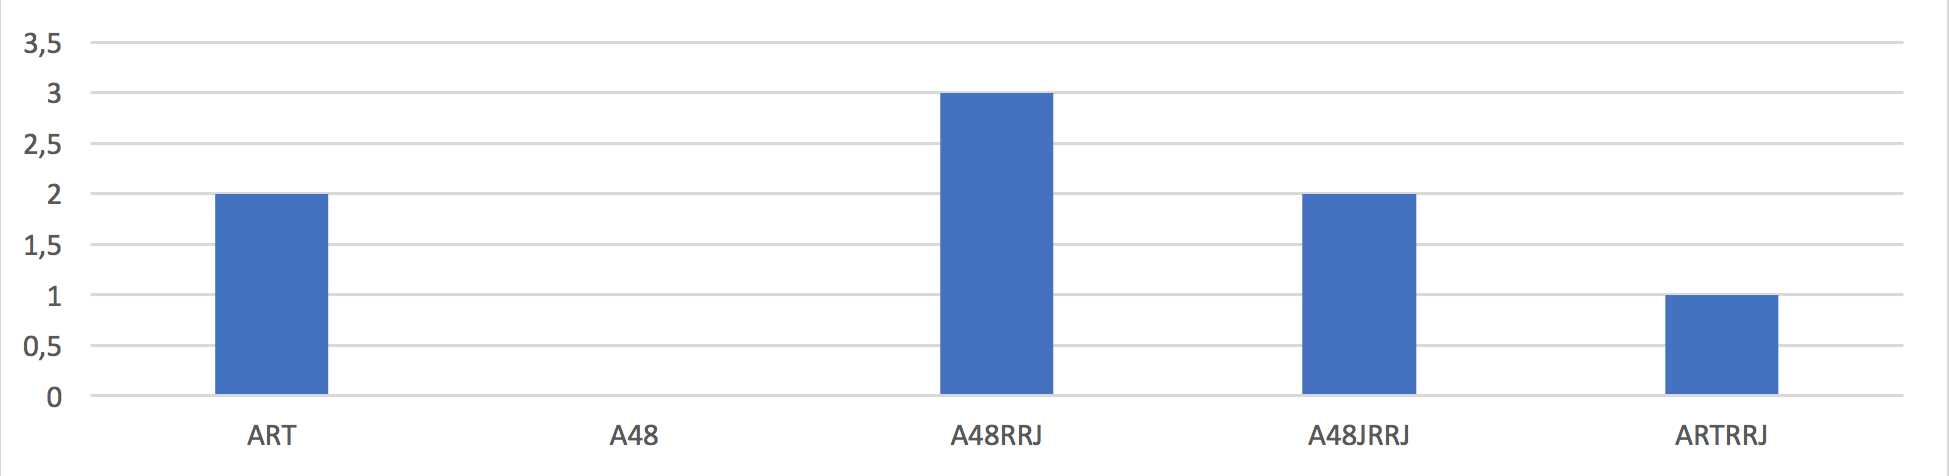
\includegraphics[width=170mm]{nivsup}
    \caption{Total de niveles superados sobre 40} % Titulo tabla en el indice
    \label{nivsup}
\end{figure}

\begin{figure}[h]
    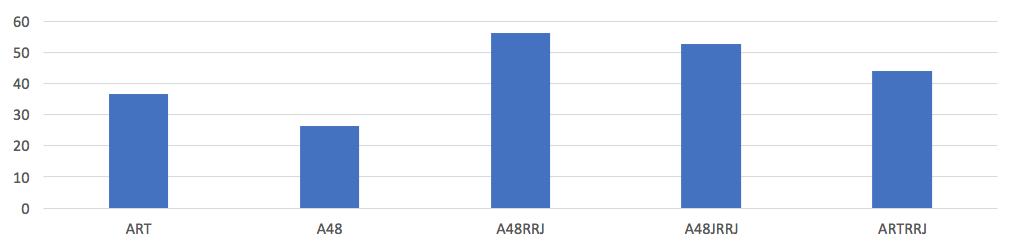
\includegraphics[width=170mm]{porcentaje}
    \caption{ Porcentaje medio de la superación en cada nivel.} % Titulo tabla en el indice
    \label{porcentaje}
\end{figure}

\begin{figure}[h]
    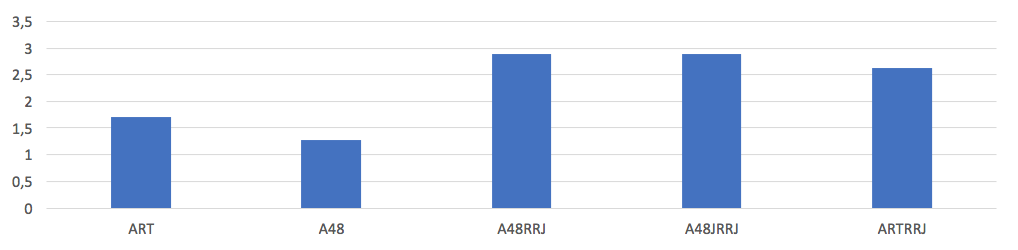
\includegraphics[width=170mm]{nivel}
    \caption{ Media de colisiones con enemigo por nivel.} % Titulo tabla en el indice
    \label{nivel}
\end{figure}

\begin{figure}[h]
    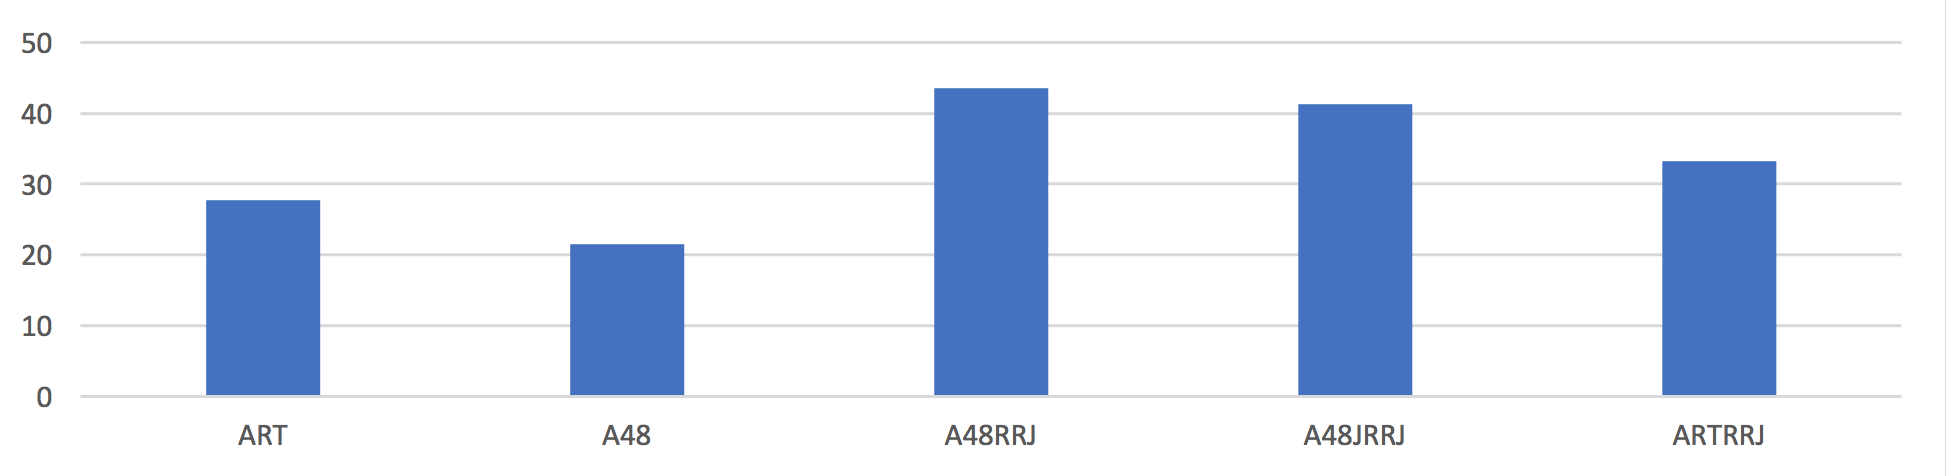
\includegraphics[width=170mm]{monedas}
    \caption{ Media de monedas recogidas por nivel.} % Titulo tabla en el indice
    \label{monedas}
\end{figure}


\begin{figure}[h]
    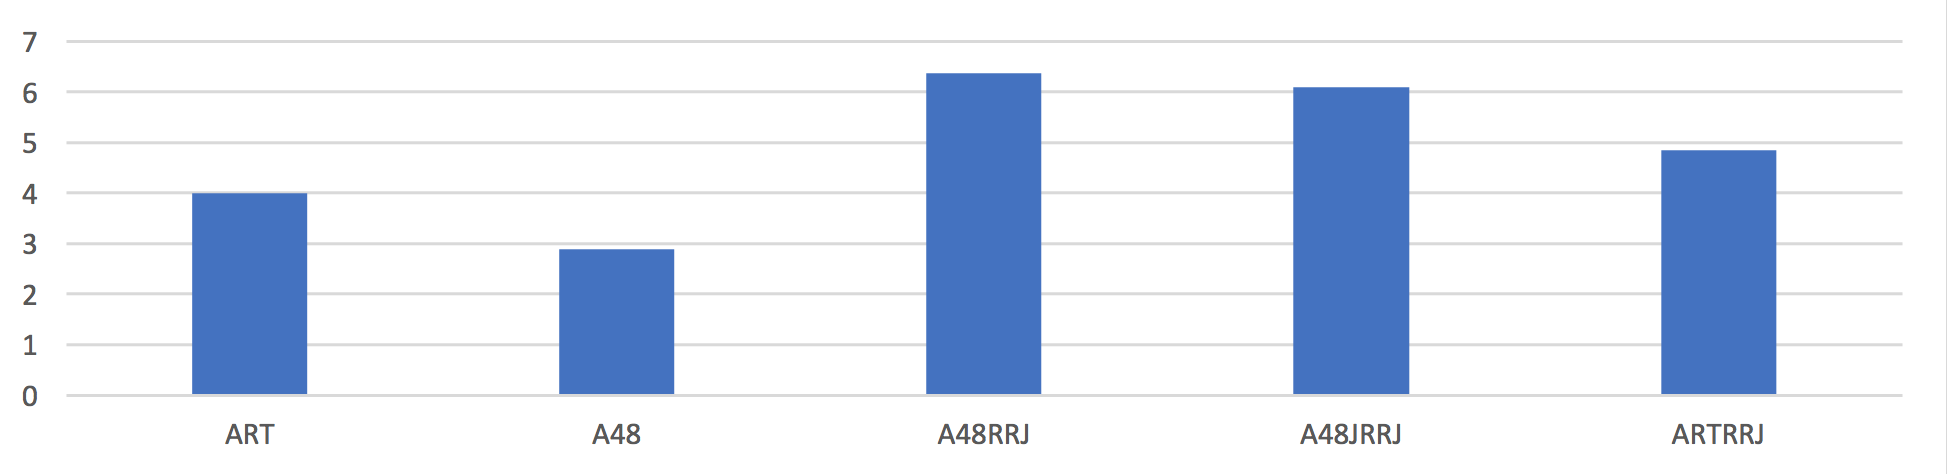
\includegraphics[width=170mm]{muertes}
    \caption{ Media de muertes de enemigos por nivel.} % Titulo tabla en el indice
    \label{muertes}
\end{figure}

\newpage
\subsection{Conclusión}
\p{
    A primera vista pareció que el ART tenía mejor desempeño, (incluso por su tendencia de no moverse en algunos niveles) pero al implementar el ARTRRJ, que también es un Random Tree pero con menos variables a clasificar, el resultado empeoró considerablemente.
    Tras unos ajustes, como se pude observar el A48RRJ es el modelo que mejor resultados ha conseguido, a pesar de sea el Agente que más colisiones posea con enemigos como se puede ver en la figura \nameref{nivel}.
    No obstante, al analizar la figura \nameref{nivel} con la figura \nameref{nivsup} podemos ver que Agentes con tasas menores de colisiones, tienen menos niveles superados. Esto se debe a que la razón de no conseguir superar el nivel no es la muerte del Agente, si no el agotamiento del tiempo debido a la dificultad encontrada para superar algunos .
}

%Falta concluir un poco más.
\newpage
\section{Regresión}\label{r}

\p{
	Para realizar la recta de regresión se cambia el objetivo, por lo que consecuentemente el preprocesado de clasificación no sirve para realizar un modelo de regresión.
	
	Consecuentemente, el único preprocesado que se va a aplicar es la selección de atributos, resultando éstos en:
\begin{itemize}
    \item \textbf{intermediateReward} 
    \item \textbf{intermediateRewardWonLast6Ticks} 
    \item \textbf{intermediaRewardPredicted12}
    \item \textbf{nearestEnemyLeftDistance}
    \item \textbf{nearestEnemyLeft\_Y}
    \item \textbf{nearestEnemyRight\_X}
    \item \textbf{nearestBlockLeftDistance}
    \item \textbf{nearestBlockLeft\_X}
    \item \textbf{nearestBlockLeft\_Y}
    \item \textbf{nearestBlockRightDistance}
    \item \textbf{nearestBlockRight\_X}
    \item \textbf{nearestBlockRight\_Y}
    \item \textbf{nearestCoinLeftDistance}
    \item \textbf{nearestCoinLeft\_X}
    \item \textbf{nearestCoinLeft\_Y}
    \item \textbf{nearestCoinRightDistance}
    \item \textbf{nearestCoinRight\_X}
    \item \textbf{nearestCoinRight\_Y}
    \item \textbf{enemyNearRight}
    \item \textbf{enemyAheadOnFloorHeight}
    \item \textbf{blockAheadOnFloorHeight}
    \item \textbf{isMarioAbleToJump}
    \item \textbf{actionKey}
    \item \textbf{intermediaRewardPredicted24}
\end{itemize}

}

\p{
	De la misma forma en la que se se han barajado los modelos de clasificación, se prueban diferentes modelos de regresión. De forma que se escoge el modelo de regresión lineal para se ser implementado debido a su elevado coeficiente de correlación entre la clase a predecir y los atributos de entrada (0.998) para n + 24.
}

\p{ 
    Para la evaluación empírica del modelo de regresión se ha implementado los tres modelos de regresión en el agente \textbf{P1BotAgentRegression}, generando datos de forma parecida a lo hecho en la sección de \nameref{a} obteniendo como resultado los siguientes tres modelos de regresión:
}\\\\
\textit{intermediaRewardPredicted24 =
     -0.282  * intermediateReward +
     -0.4332 * intermediateRewardWonLast6Ticks +
      1.2849 * intermediaRewardPredicted12 +
      0.1646 * nearestEnemyLeftDistance +
     -0.4056 * nearestEnemyLeft\_Y +
     -1.0682 * nearestEnemyRightDistance +
      0.7969 * nearestEnemyRight\_X +
     -2.3371 * nearestBlockLeftDistance +
     -0.6307 * nearestBlockLeft\_X +
     -1.315  * nearestBlockLeft\_Y +
     -0.3964 * nearestBlockRightDistance +
      0.5082 * nearestBlockRight\_X +
     -2.9267 * nearestCoinLeftDistance +
     -0.3925 * nearestCoinLeft\_X +
     -0.6596 * nearestCoinLeft\_Y +
     -0.428  * nearestCoinRightDistance +
      0.5277 * nearestCoinRight\_X +
     -0.063  * nearestCoinRight\_Y +
     -1.36   * enemyNearRight +
      2.7432 * enemyAheadOnFloorHeight +
     -0.6076 * blockAheadOnFloorHeight +
     -2.2931 * isMarioAbleToJump +
      4.3648 * enemyWasKilledBin +
     -1.4951 * actionKey +
     62.1584}\\\\
     \textit{intermediaRewardPredicted12 =
     -0.5811 * intermediateReward +
     -0.175  * intermediateRewardWonLastTick +
     -0.3572 * intermediateRewardWonLast6Ticks +
      1.2906 * intermediaRewardPredicted6 +
      0.29   * intermediaRewardPredicted24 +
     -0.0693 * nearestEnemyLeftDistance +
     -0.3781 * nearestEnemyLef\_X +
      0.1532 * nearestEnemyLeft\_Y +
     -0.1737 * nearestEnemyRightDistance +
      0.1261 * nearestEnemyRight\_X +
      0.1246 * nearestEnemyRight\_Y +
      0.8084 * nearestBlockLeftDistance +
      0.6317 * nearestBlockLeft\_X +
      0.441  * nearestBlockLeft\_Y +
     -0.0942 * nearestBlockRight\_X +
      0.5381 * nearestCoinLeftDistance +
      0.4871 * nearestCoinLeft\_X +
      0.1769 * nearestCoinLeft\_Y +
      0.0948 * nearestCoinRightDistance +
      0.9151 * enemyNearRight +
     -0.6406 * blockAheadOnFloorHeight +
     -1.2063 * isMarioOnGround +
      0.5919 * isMarioAbleToJump +
      0.8761 * coinsGainedLastTick +
      0.538  * actionKey +
    -19.2973}\\\\
    \textit{intermediaRewardPredicted6 =
    1      * intermediateReward +
   -0.0008 * intermediateRewardWonLastTick +
    1.0001 * intermediateRewardWonLast6Ticks +
    0.0001 * intermediaRewardPredicted12 +
   -0.0001 * intermediaRewardPredicted24 +
   -0.0058 * nearestEnemyLeftDistance +
   -0.0068 * nearestEnemyLef\_X +
   -0.0039 * nearestEnemyLeft\_Y +
    0.014  * nearestEnemyRightDistance +
   -0.0106 * nearestEnemyRight\_X +
   -0.0024 * nearestBlockLeftDistance +
   -0.0032 * nearestBlockLeft\_X +
   -0.0035 * nearestBlockLeft\_Y +
    0.0044 * nearestBlockRightDistance +
   -0.0042 * nearestBlockRight\_X +
    0.0033 * nearestBlockRight\_Y +
   -0.0007 * nearestCoinLeftDistance +
   -0.0013 * nearestCoinLeft\_Y +
    0.0012 * nearestCoinRightDistance +
   -0.0016 * nearestCoinRight\_X +
    0.0002 * nearestCoinRight\_Y +
    0.0307 * enemyNearRight +
    0.013  * blockNearRight +
    0.0167 * enemyAheadOnFloorHeight +
   -0.01   * blockAheadOnFloorHeight +
   -0.015  * isMarioOnGround +
   -0.0145 * isMarioAbleToJump +
   -0.0105 * enemyWasKilledBin +
    0.0173 * coinsGainedLastTick +
   -0.0561 * actionKey +
    0.384}
\newpage
\p{Tras su ejecución en MarioAi, hemos obtenido los siguientes resultados:}\\\\
\texttt{\#\#\#\#\#\#\#\# Resultados de la regresión: \#\#\#\#\#\#\#\#\\\\
\#\#\#\# Predicted n + 6 \#\#\#\#\\
        De un total de 922 ticks ha predicho correctamente 13 ticks (0.0\%) y 903 ticks erróneamente (100.0\%).\\
        La acumulación de intermediateReward predicha ha sido 940128 y el valor real es de 928074, lo que nos da una desviación de 12054\\\\
        \#\#\#\# Predicted n + 12 \#\#\#\#\\
        De un total de 922 ticks ha predicho correctamente 0 ticks (100.0\%) y 910 ticks erróneamente (0.0\%).\\
        La acumulación de intermediateReward predicha ha sido 951316 y el valor real es de 928074, lo que nos da una desviación de 23242\\\\
        \#\#\#\# Predicted n + 24 \#\#\#\#\\
        De un total de 922 ticks ha predicho correctamente 0 ticks (100.0\%) y 898 ticks erróneamente (0.0\%).\\
        La acumulación de intermediateReward predicha ha sido 968758 y el valor real es de 928074, lo que nos da una desviación de 40684}

    %TODO: resultados
\newpage
\section{Implementación}\label{i}
\p{
    Para la implementación del árbol decisión en MarioAI se ha utilizado la herramienta weka para el preporocesado de los datos y la generación resultante. Un árbol resultante de weka podría tener el siguiente aspecto:\\
    \begin{lstlisting}[language=Java]
        blockNearRight = 0
        |   nearestEnemyRight_X < 11.5 : 2 (1758/36)
        |   nearestEnemyRight_X >= 11.5 : 2 (4541/35)
        blockNearRight = 1
        |   nearestEnemyRight_Y < 12.5 : 2 (763/353)
        |   nearestEnemyRight_Y >= 12.5 : 2 (260/85)
    \end{lstlisting}
    Estos modelos son fácilmente traspasables a la plataforma MarioAI siempre que no tengan un excesivo tamaño. Fácilmente traspasable código java, siguiendo el ejemplo anterior.
    \begin{lstlisting}[language=Java]
        if(this.blockNearRight == 0){
            if(this.nearestEnemyRight_X < 11.5){ 
                action[Mario.KEY_RIGHT] = true;
            }else{
                action[Mario.KEY_RIGHT] = true;
            }
        }else{
            if(this.nearestEnemyRight_Y < 12.5){
                action[Mario.KEY_RIGHT] = true;
            }else{
                action[Mario.KEY_RIGHT] = true;
            }
        }
     \end{lstlisting}
}

\section{Opiniones Personales}
Esta práctica es una simple visualización de la aplicación de técnicas de Aprendizaje Automático. No obstante, la carga de trabajo sumada a las previas entregas hace que la asignatura requiera más horas deseadas, haciendo que la calidad de trabajo tenga que ser disminuida. 
No obstante, al ser una práctica tan visual, resulta muy desafiante conseguir buenos resultados, lo que la hace ligera y bien llevadera. 
De esta práctica, se debería de mejorar el apartado de predicción, pues para es conceptualmente diferente al resto de la práctica, y no ha quedado claro el enfoque que se debe de tomar en ese apartado.
\end{document}